%%%%%%%%%%%%%%%%%%%%%%%%%%%%%%%%%%%%%%%%%%%%%%%%%%%%%%%%%%%%%%%%%%%%%%%%%%%%%
\chapter{Practical Part}\label{chap:practicalPart}
%%%%%%%%%%%%%%%%%%%%%%%%%%%%%%%%%%%%%%%%%%%%%%%%%%%%%%%%%%%%%%%%%%%%%%%%%%%%%
\chapterstart

TODO: Your text here \ldots
\section{Use Case}
This use case is entirely fictional but allows the reader to get a better understanding of the circumstances a that led to the design of a federated authentication solution. The scenario features a medium to large company with up to 1000 employees. The mission of the company is to provide a network and analyzing toolset which allows the customer of the product suite to improve security within his network and keep an overview of potential security risks. Previously the customers received monthly reports about their current state of the network. Each of the products and tools resulted in a separate report which was sent via E-Mail. To modernize the approach, the reports should be replaced by a modern single-page application that could be accessed by customers and by employees for administrative reasons. In this example, we call the solution 'Security Assessment Portal.' The Security Assessment Portal should give the customers an overview of current products and the performance of the network an example of the suit could be E-Mail-filtering.  

The company already has a particular set of internal applications that are used by the employees within the company network. The company internally uses active directory for authorization on local machines. All applications until now are accessible within the companies network and use windows authentication. The application should be accessible by employees as well as customers whereas customers should not receive access to the company network. The data of the customers are sensible and therefore worth protecting. Because of the highly sensible data, certain customer do not need which to authenticate with an external provider. The application should be hosted within the company a solution for customers to access the application from outside is needed.


\section{Risk Assessment}

Risk Assessment is one of the essential elements when it comes to managing risks of an organization. The aim of risk assessment is it to identify, estimate, and prioritize risk to operations, assets, individuals, other organizations from the operations and use of the information system. The risks assessment should help to make decisions on how to respond to certain risk. The steps to a risk assessment are identifying potential threats, internal and external vulnerabilities, the impact to organizations given the potential for threats exploiting vulnerabilities and the likelihood of that harm to occur. There are three tiers according to (\cite{NIST:2012:GCRA}, p.1) in risk management:

\begin{itemize}
	\item Tier 1 - organizational level
	\item Tier 2 - mission/business process level
	\item Tier 3 - information system level
\end{itemize}

The first two Tiers are focusing on risks related to organizational governance and management activities, mission/business processes, enterprise architecture or the funding of information security programs. The third Tier focuses more on how to implement a risk management framework successfully [cf. (\cite{NIST:2012:GCRA}, p.1)]. 

To prepare for a risk assessment, it helps to identify the purpose, scope, assumptions, and constraints beforehand. The purpose of this risk assessment is to make authorization-related decisions and conducting an initial assessment to identify potential threats, internal and external vulnerabilities, impact to organizations. The scope addresses the 3 Tier. The focal point is the risk assessment of a single sign-on federation system. Furthermore, the scope is defined by what the result is expected from the risk assessment. In this risk assessment, an authentication and authorization solution is needed for a specific use case. The assessment result should usually be reevaluated after the initial draft [cf. (\cite{NIST:2012:GCRA}, pp.24)].

Typically a risk assessment is a very complex task that takes a lot of time an many external sources to be representative, like for example expert opinions. If put together correctly one should end up with a Risk Management Framework (RMF). A RMF provides a process that integrates security and risk management activities into the system development life cycle. The system can be applied to both new and legacy systems. \cite{NIST:2018:RMF} defines 6 Steps in this RMF. The steps are Categorize, Select, Implement, Assess, Authorize and Monitor [cf. (\cite{NIST:2018:RMF})]. 

However since a full RMF is out of the scope a scaled down version that is specific to digital identity risk management is conducted. Modern digital services often combine identity proofing, authentication and federation requirements in one single bundle. It is better to look at each of this components separately to delivery the best identity service [cf. (\cite{NIST:2017:DIG})].  

TODO: Your text here ...


\section{Solution}
The \cite{Sakimura:2014:OpenIDConnect} explains that modern applications have different requirements than their predecessor due to new distributed architectures that allow enterprises to be more flexible. Cloud or Microservice architectures require different interactions between applications as the \ref{fig:architecture-identityserver} below show the most common interactions for modern applications.

\begin{figure}[h]
	\centering
	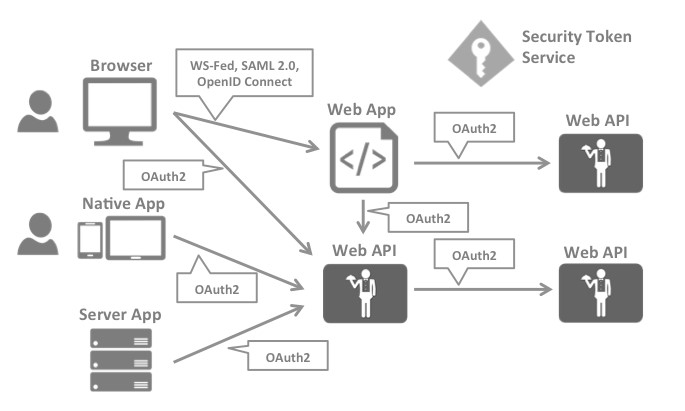
\includegraphics[width=0.8\linewidth]{images/architecture-identityserver}
	\caption[Architecture IdentityServer4]{}
	\caption{}
	\label{fig:architecture-identityserver}
\end{figure}



For example, a browser might call a Web App, and a Web App calls a Web API or perhaps a Native App calls a Web API, which is calling another Web API. Each application has to implement security functions to maintain a secure flow throughout these interactions, Implementing this security features for each involved application leads to a lot of duplicated code and inconsistencies. A different approach to implement security throughout these flows is using a token service. A token service brings the benefit of being able to encapsulate these security functions. Security functions can be updated and hosted at a single point which prevents duplicated functions across applications and security flaws [cf. (\cite{Sakimura:2014:OpenIDConnect})].

Identity Server4 is an ASP.NET framework that uses the specifics of OpenID Connect and OAuth 2.0 to enable Authentication and Authorization related features. Features include Authentication as a Service, which provides a centralized login logic for all applications, Single sign-on, Access Control for APIs and Federation Gateway. The Identity Server 4 will be used as a Token Server in the practical part [cf. (\cite{Brock:2018:ID4})]

The project illustrating the use of Identity Server and the benefits of OpenID Connect an OAuth is a Visual Studio Project mostly written in C\# and Typescript. The project example for Identity Server includes four different projects:

\begin{itemize}
	\item Identity Server - The Identity Server is a ASP.NET Core Project with basic Implementation of an Identity Server which serves as a Token Server. 
	\item ProjectApiNetCore - This application is a ASP.NET Core 2.0 API Application with basic API that returns the users Claims if he is authenticated.
	\item Angular Client - The Angular Client is a ASP.NET Core MVC Angular Project used as a Client that can be accessed by an End-User who can authenticate with the Identity Server and requests protected resources of the API ProjectApiNetCore.This project uses the Implicit Code Flow. 
	\item MVC Client - The MVC Client is a ASP.NET Core MVC Project used as a Client that can be accessed by an End-User and can authenticate with the Identity Server and requests protected resources of the API ProjectApiNetCore. This project uses the Hybrid Code Flow. 
\end{itemize}



\paragraph{Identity Server}

This project is using the IdentityServer4 library by Brock Allen and Dominick Baier. The Project works as a Token Server which means that the Identity Server Project is responsible for authentication the user, managing the identities and provide and approve tokens. Furthermore, the Identity Server implements different Authentication Flows.


\begin{figure}[h]
	\centering
	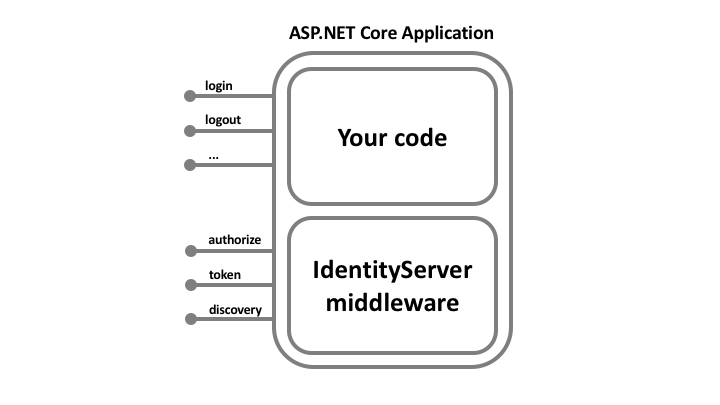
\includegraphics[width=0.7\linewidth]{images/middlewareIdentityServer}
	\caption{IdentityServer Middleware}
	\label{fig:middlewareidentityserver}
\end{figure}
 

IdentityServer4 adds endpoints of OAuth 2.0 and OpenID Connect to an arbitrary ASP.NET Core application as shown in \ref{fig:middlewareidentityserver}. The identity server can be as complex as the developer wants but \cite{Brock:2018:ID4} recommends to keep the attack surface as small as possible by just including authentication related UI only [cf. (\cite{Brock:2018:ID4})]. 


For the basic Setup, the Identity Server has to be added to the StartUp class and to ensure a secure communication a certificate has is created to sign the request. For the basic setup, Identity Server provides us with DeveloperSigningCredentials which provides a dummy certificate. In this example application, a real certificate is included. 

\begin{figure}[h]
	\centering
	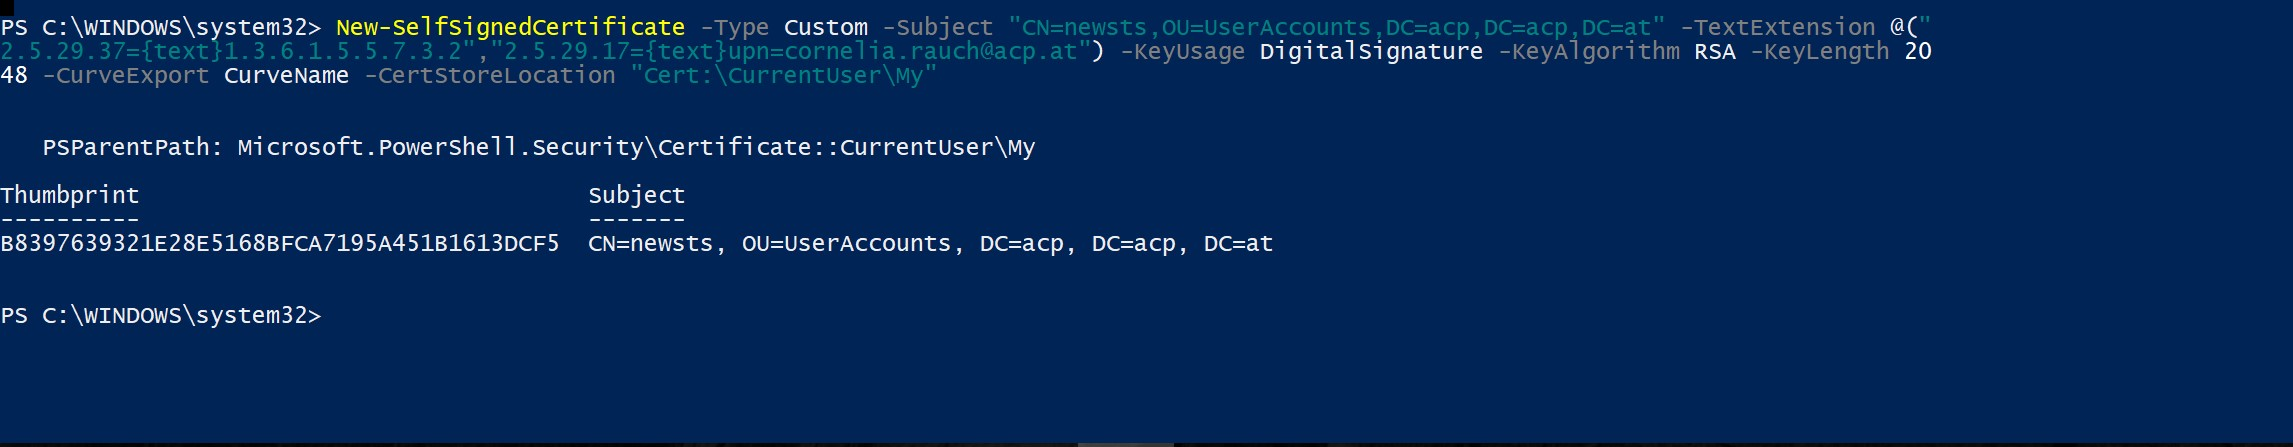
\includegraphics[width=0.8\linewidth]{images/self-signed-certicate}
	\caption{Self signed Certicate with Powershell}
	\label{fig:self-signed-certicate}
\end{figure}

The certificate used in this application was created with Powershell as shown in \ref{fig:self-signed-certicate}. The algorithm used in this certificate is RSA. Depending on the algorithm that is used in the certificate a similar hashing algorithm has to be used for the Client Secret.


The API Resources include the available APIs that can be called and included in the scope of a request. The Identity Resources are Resources that can be included in the returning id\_token. The Clients are the available Clients that can be configured and can use the Identity Server. Those Client Configurations indicate which Authorization Flow is used and how to retrieve id\_token, access\_token, and a possible refreh\_token. For simplifying reasons, Identity Server provides an in Memory User Storage which can be used for Testing reasons. Other ways to define Users are via .NET Core Identity or IdentityServer4 EntityFramework. For the purpose of this implementation this Test Users where included in the Identity Server application:
\begin{enumerate}
	\item User1:
	\begin{itemize}
		\item  Username: bob
		\item  Password: bob
	\end{itemize} 
	\item User2:
	\begin{itemize}
		\item  Username: alice
		\item  Password: alice
	\end{itemize} 
\end{enumerate}

After the basic setup of the Identity Server, it can be examined if the Identity Server is running correctly by calling the discovery document. The discovery document can be used by the Clients and APIs to retrieve necessary configuration data. The Identity Server has to run at local port 5000 and in the browser navigate to
\url{http://localhost:5000/.well-known/openid-configuration}.

\begin{figure}[h]
	\centering
	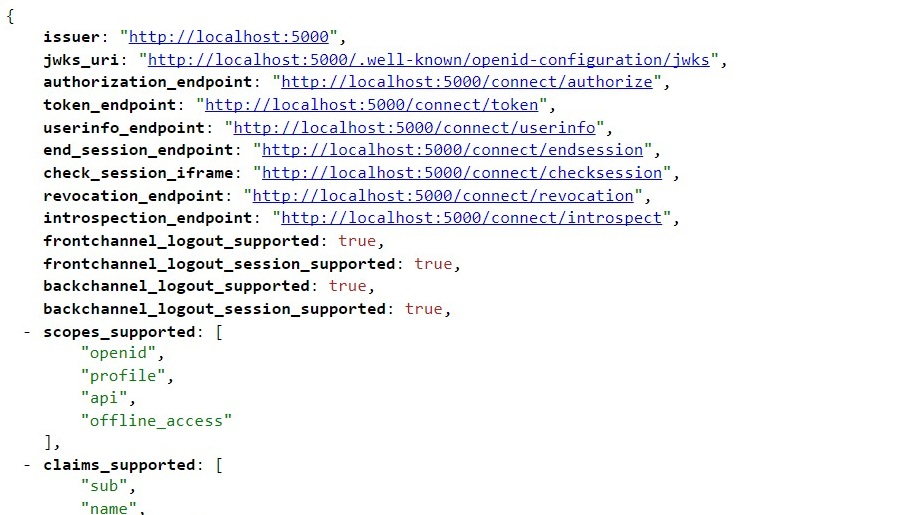
\includegraphics[width=0.8\linewidth]{images/openid-discovery-document}
	\caption{OpenID Discovery Document}
	\label{fig:openid-discovery-document}
\end{figure}
The discovery document is located at a well-known location and is containing key-value pairs as a JSON structure. The key-value pairs int he discovery document represent multiple endpoints that are used to authenticate a user including URIs of the authorization, token, userinfo, and public-keys endpoint. The use of a discovery document brings more flexibility to the protocol brings more flexibility. The application should have the discovery URL hard-coded in the application according to (\cite{Google:2018:IdentityPlatform}) the discovery document URL can then be used to fetch endpoints from the document and use them to for example send an authentication request [cf. (\cite{Google:2018:IdentityPlatform})].

The metadata that is seen in \ref{fig:openid-discovery-document} OpenID discovery document is a mixture of required elements with some recommended ones that are implemented by the identity server. The required elements are issuer, authorization\_endpoint, token\_endpoint, jwks\_uri, response\_types\_supported, subject\_types\_supported and id\_token\_signing\_alg\_supported. The issuer, in this case, is this Identity Servers address. The authorization\_endpoint is the URL OAuth 2.0 Authorization Endpoint. The user is redirected to the authorization server's authorization endpoint for authentication and authorization. The authentication request that is sent to the authorization server can have different request parameters. These request parameters are defined by OAuth 2.0 and additional request parameters defined by OpenID Connect. The token\_endpoint is the URL of the OAuth 2.0 Token Endpoint. The RP can request access or optionally refresh tokens from the token endpoint. The user\_endpoint can be used to request additional information concerning the user. The response\_types\_supported is important information about what kind of response is supported and ultimately what kind of authentication flow can be used based on that information like described in chapter \ref{chap:authenticationandauthorization} in Single-Sign on Federate Systems. The subject\_types\_supported is a list of subject identifier types. Moreover, last but not least id\_token\_signing\_alg\_supported is used to find out which JWS is signing algorithm is used to encode the ID token and get the claims of the JWT. The algorithm RS256 must be included [cf. (\cite{Sakimura:OIDCC}, (\cite{Sakimura:OIDCD}))].. 

\begin{figure}[h]
	\centering
	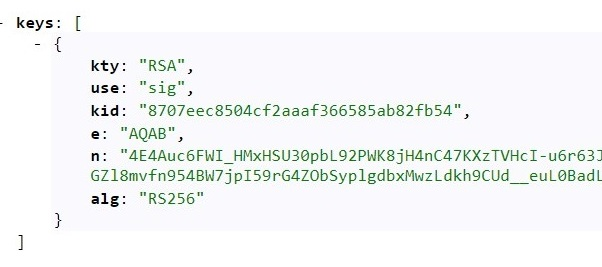
\includegraphics[width=0.7\linewidth]{images/jwkDiscovoryDocument}
	\caption{JWKS Endpint}
	\label{fig:jwkdiscovorydocument}
\end{figure}

The jwks\_endpoint is worth a closer look. JWKS SET is published to the JWKS endpoint. The keys shown in (\ref{fig:jwkdiscovorydocument} JWKS Endpoint) can be rolled over by periodically adding new keys to the JWK Set. This also indicates if the cryptographic algorithms are configured correctly. E.g. : The message is using the kid of signing key in the JOSE Header to indicate which key has to be used to validate the signature. The algorithm used by the signing party has to be supported by the recipient and can be either and Asymmetric Signature or a Symmetric Signature. 
When using RSA or ECDSA signatures, the alg Header Parameter has to be set to the correct algorithm, and the private key used to sign must be associated with the public key published by the sender. When using MAC-based signatures, the alg Header Parameter has to be set to the correct algorithm, and the MAC key is the octets of the UTF-8 representation of the client\_secret. MAC-based signatures cannot be used by public Clients because they cannot keep secrets.  All metadata types are listed in the specification of OpenID Discovery Document from \cite{Sakimura:OIDCD} [cf. (\cite{Sakimura:OIDCC}, (\cite{Sakimura:OIDCD}))]. 

After calling the OpenID discovery document and the JWKS endpoint, one can be ensured that the basic setup of the IdentityServer works. Next, a resource that is worth beeing protected by the Identity Server has to be created. 

\paragraph{ProjectApiNetCore}

This ProcjectApiNetcore is an ASP.NET Core application. This application represents the Resource Server and serves the Protected Resources. In this particular example, the API provides a list of Products the user bought from the company and the possibility to download the report that gives information about the current state of the product. The example API provides dummy data for the particular request. For easy testing of the API and designing the API, swagger.io is used. Furthermore, swagger.io (\url{https://swagger.io/}) gives a nice developer experience with an interactive API documentation. In addition, it is possible to generate code out of the swagger documentation for different programming languages with tools like NSwag (\url{https://github.com/RSuter/NSwag}).

\begin{figure}[h]
	\centering
	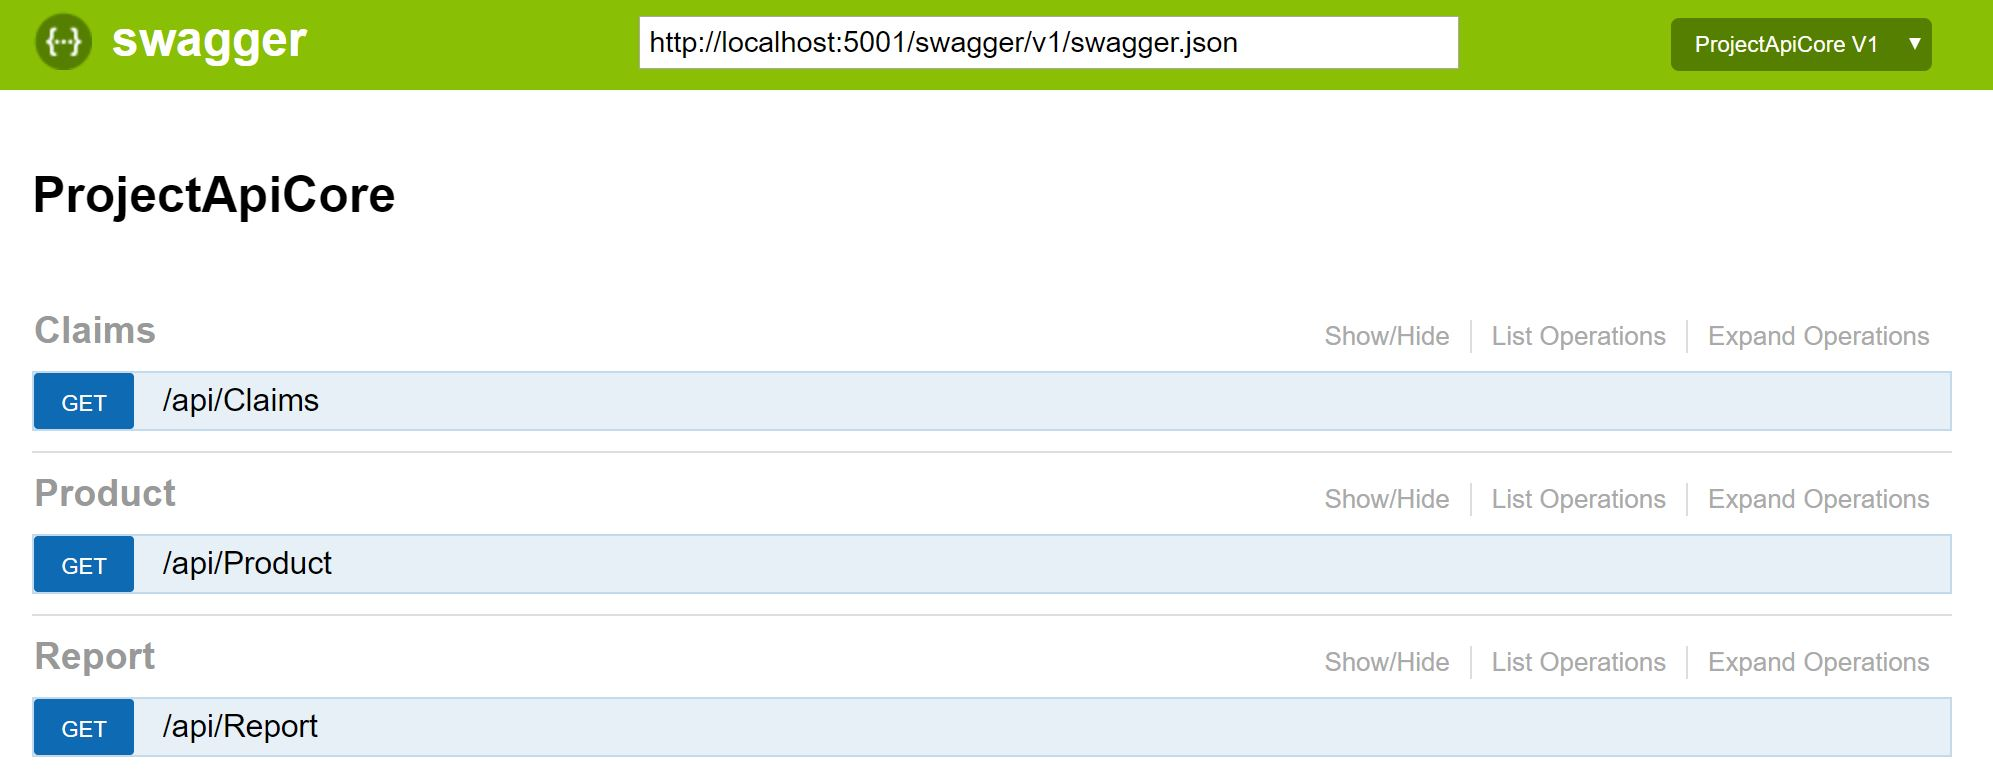
\includegraphics[width=0.7\linewidth]{images/apis}
	\caption{API documentation with Swagger}
	\label{fig:apis}
\end{figure}

All of the routes shown in \ref{fig:apis} API documentation with Swagger, are secured with the help of the IdentityServer4.AccessTokenValidation NuGet package. Each Controller gets an Authorize annotation. 
To configure the right authentication method, ASP.NET Core 2.0 offers the possibility to add the authentication to the pipeline with Dependency Injection via the method Configure Services in the Startup.class.
In the StartUp class of the API Project the AddAuthentication with the Value "JwtBearerDefaults.AuthenticationSchemeMakes "Bearer" the default authentication scheme “Bearer”. With the AddIdentityServerAuthentication it is defined which Token server can be used to validate the incoming token and make sure that this token is from a trusted issuer. It adds the Identity Server access token validation handler into DI and also it is checked if the token is valid to be used with this API (aka scope). Adding UseAuthentication to the Configure method int the Startup class adds the authentication middleware to the pipeline so authentication will be performed automatically on every call into the host.  Multiple authentication schemes can be used. A list of authentication schemes is then passed to the Authorize attribute separated with a comma. The default scheme results in the HttpContext.User property is set to that identity. After adding the Authentication logic to the API Project, the resources should be protected know. To check if the resources are protected the Swagger documentation can be used. Therefore one has to navigate to \url{http://localhost:5001/swagger/v1/swagger.json} and try out one of the methods shown in (\ref{fig:apis}) API Documentation with Swagger. This should result in a 401 Unauthorized HTTP response code.

 

TODO: Your text here...

\chapterend
